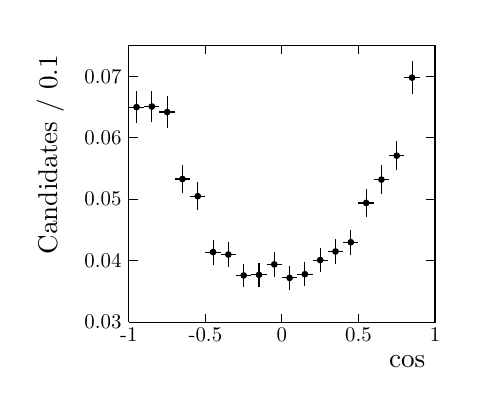
\begin{tikzpicture}
\pgfdeclareplotmark{cross} {
\pgfpathmoveto{\pgfpoint{-0.3\pgfplotmarksize}{\pgfplotmarksize}}
\pgfpathlineto{\pgfpoint{+0.3\pgfplotmarksize}{\pgfplotmarksize}}
\pgfpathlineto{\pgfpoint{+0.3\pgfplotmarksize}{0.3\pgfplotmarksize}}
\pgfpathlineto{\pgfpoint{+1\pgfplotmarksize}{0.3\pgfplotmarksize}}
\pgfpathlineto{\pgfpoint{+1\pgfplotmarksize}{-0.3\pgfplotmarksize}}
\pgfpathlineto{\pgfpoint{+0.3\pgfplotmarksize}{-0.3\pgfplotmarksize}}
\pgfpathlineto{\pgfpoint{+0.3\pgfplotmarksize}{-1.\pgfplotmarksize}}
\pgfpathlineto{\pgfpoint{-0.3\pgfplotmarksize}{-1.\pgfplotmarksize}}
\pgfpathlineto{\pgfpoint{-0.3\pgfplotmarksize}{-0.3\pgfplotmarksize}}
\pgfpathlineto{\pgfpoint{-1.\pgfplotmarksize}{-0.3\pgfplotmarksize}}
\pgfpathlineto{\pgfpoint{-1.\pgfplotmarksize}{0.3\pgfplotmarksize}}
\pgfpathlineto{\pgfpoint{-0.3\pgfplotmarksize}{0.3\pgfplotmarksize}}
\pgfpathclose
\pgfusepathqstroke
}
\pgfdeclareplotmark{cross*} {
\pgfpathmoveto{\pgfpoint{-0.3\pgfplotmarksize}{\pgfplotmarksize}}
\pgfpathlineto{\pgfpoint{+0.3\pgfplotmarksize}{\pgfplotmarksize}}
\pgfpathlineto{\pgfpoint{+0.3\pgfplotmarksize}{0.3\pgfplotmarksize}}
\pgfpathlineto{\pgfpoint{+1\pgfplotmarksize}{0.3\pgfplotmarksize}}
\pgfpathlineto{\pgfpoint{+1\pgfplotmarksize}{-0.3\pgfplotmarksize}}
\pgfpathlineto{\pgfpoint{+0.3\pgfplotmarksize}{-0.3\pgfplotmarksize}}
\pgfpathlineto{\pgfpoint{+0.3\pgfplotmarksize}{-1.\pgfplotmarksize}}
\pgfpathlineto{\pgfpoint{-0.3\pgfplotmarksize}{-1.\pgfplotmarksize}}
\pgfpathlineto{\pgfpoint{-0.3\pgfplotmarksize}{-0.3\pgfplotmarksize}}
\pgfpathlineto{\pgfpoint{-1.\pgfplotmarksize}{-0.3\pgfplotmarksize}}
\pgfpathlineto{\pgfpoint{-1.\pgfplotmarksize}{0.3\pgfplotmarksize}}
\pgfpathlineto{\pgfpoint{-0.3\pgfplotmarksize}{0.3\pgfplotmarksize}}
\pgfpathclose
\pgfusepathqfillstroke
}
\pgfdeclareplotmark{newstar} {
\pgfpathmoveto{\pgfqpoint{0pt}{\pgfplotmarksize}}
\pgfpathlineto{\pgfqpointpolar{44}{0.5\pgfplotmarksize}}
\pgfpathlineto{\pgfqpointpolar{18}{\pgfplotmarksize}}
\pgfpathlineto{\pgfqpointpolar{-20}{0.5\pgfplotmarksize}}
\pgfpathlineto{\pgfqpointpolar{-54}{\pgfplotmarksize}}
\pgfpathlineto{\pgfqpointpolar{-90}{0.5\pgfplotmarksize}}
\pgfpathlineto{\pgfqpointpolar{234}{\pgfplotmarksize}}
\pgfpathlineto{\pgfqpointpolar{198}{0.5\pgfplotmarksize}}
\pgfpathlineto{\pgfqpointpolar{162}{\pgfplotmarksize}}
\pgfpathlineto{\pgfqpointpolar{134}{0.5\pgfplotmarksize}}
\pgfpathclose
\pgfusepathqstroke
}
\pgfdeclareplotmark{newstar*} {
\pgfpathmoveto{\pgfqpoint{0pt}{\pgfplotmarksize}}
\pgfpathlineto{\pgfqpointpolar{44}{0.5\pgfplotmarksize}}
\pgfpathlineto{\pgfqpointpolar{18}{\pgfplotmarksize}}
\pgfpathlineto{\pgfqpointpolar{-20}{0.5\pgfplotmarksize}}
\pgfpathlineto{\pgfqpointpolar{-54}{\pgfplotmarksize}}
\pgfpathlineto{\pgfqpointpolar{-90}{0.5\pgfplotmarksize}}
\pgfpathlineto{\pgfqpointpolar{234}{\pgfplotmarksize}}
\pgfpathlineto{\pgfqpointpolar{198}{0.5\pgfplotmarksize}}
\pgfpathlineto{\pgfqpointpolar{162}{\pgfplotmarksize}}
\pgfpathlineto{\pgfqpointpolar{134}{0.5\pgfplotmarksize}}
\pgfpathclose
\pgfusepathqfillstroke
}
\definecolor{c}{rgb}{1,1,1};
\draw [color=c, fill=c] (0.1,0.0925676) rectangle (4.9,4.53581);
\draw [color=c, fill=c] (0.772,0.803486) rectangle (4.66,4.31365);
\definecolor{c}{rgb}{0,0,0};
\draw [c] (0.772,0.803486) -- (0.772,4.31365) -- (4.66,4.31365) -- (4.66,0.803486) -- (0.772,0.803486);
\draw [c,line width=0.4] (0.8692,3.33474) -- (0.8692,3.53361);
\draw [c,line width=0.4] (0.8692,3.53361) -- (0.8692,3.73248);
\draw [c,line width=0.4] (0.772,3.53361) -- (0.8692,3.53361);
\draw [c,line width=0.4] (0.8692,3.53361) -- (0.9664,3.53361);
\foreach \P in {(0.8692,3.53361)}{\draw[mark options={color=c,fill=c},mark size=1.201201pt,mark=*,mark size=1pt] plot coordinates {\P};}
\draw [c,line width=0.4] (1.0636,3.34239) -- (1.0636,3.54141);
\draw [c,line width=0.4] (1.0636,3.54141) -- (1.0636,3.74044);
\draw [c,line width=0.4] (0.9664,3.54141) -- (1.0636,3.54141);
\draw [c,line width=0.4] (1.0636,3.54141) -- (1.1608,3.54141);
\foreach \P in {(1.0636,3.54141)}{\draw[mark options={color=c,fill=c},mark size=1.201201pt,mark=*,mark size=1pt] plot coordinates {\P};}
\draw [c,line width=0.4] (1.258,3.27357) -- (1.258,3.47121);
\draw [c,line width=0.4] (1.258,3.47121) -- (1.258,3.66885);
\draw [c,line width=0.4] (1.1608,3.47121) -- (1.258,3.47121);
\draw [c,line width=0.4] (1.258,3.47121) -- (1.3552,3.47121);
\foreach \P in {(1.258,3.47121)}{\draw[mark options={color=c,fill=c},mark size=1.201201pt,mark=*,mark size=1pt] plot coordinates {\P};}
\draw [c,line width=0.4] (1.4524,2.44089) -- (1.4524,2.62097);
\draw [c,line width=0.4] (1.4524,2.62097) -- (1.4524,2.80106);
\draw [c,line width=0.4] (1.3552,2.62097) -- (1.4524,2.62097);
\draw [c,line width=0.4] (1.4524,2.62097) -- (1.5496,2.62097);
\foreach \P in {(1.4524,2.62097)}{\draw[mark options={color=c,fill=c},mark size=1.201201pt,mark=*,mark size=1pt] plot coordinates {\P};}
\draw [c,line width=0.4] (1.6468,2.22727) -- (1.6468,2.40256);
\draw [c,line width=0.4] (1.6468,2.40256) -- (1.6468,2.57785);
\draw [c,line width=0.4] (1.5496,2.40256) -- (1.6468,2.40256);
\draw [c,line width=0.4] (1.6468,2.40256) -- (1.744,2.40256);
\foreach \P in {(1.6468,2.40256)}{\draw[mark options={color=c,fill=c},mark size=1.201201pt,mark=*,mark size=1pt] plot coordinates {\P};}
\draw [c,line width=0.4] (1.8412,1.53401) -- (1.8412,1.69273);
\draw [c,line width=0.4] (1.8412,1.69273) -- (1.8412,1.85144);
\draw [c,line width=0.4] (1.744,1.69273) -- (1.8412,1.69273);
\draw [c,line width=0.4] (1.8412,1.69273) -- (1.9384,1.69273);
\foreach \P in {(1.8412,1.69273)}{\draw[mark options={color=c,fill=c},mark size=1.201201pt,mark=*,mark size=1pt] plot coordinates {\P};}
\draw [c,line width=0.4] (2.0356,1.50358) -- (2.0356,1.66153);
\draw [c,line width=0.4] (2.0356,1.66153) -- (2.0356,1.81947);
\draw [c,line width=0.4] (1.9384,1.66153) -- (2.0356,1.66153);
\draw [c,line width=0.4] (2.0356,1.66153) -- (2.1328,1.66153);
\foreach \P in {(2.0356,1.66153)}{\draw[mark options={color=c,fill=c},mark size=1.201201pt,mark=*,mark size=1pt] plot coordinates {\P};}
\draw [c,line width=0.4] (2.23,1.24506) -- (2.23,1.39631);
\draw [c,line width=0.4] (2.23,1.39631) -- (2.23,1.54757);
\draw [c,line width=0.4] (2.1328,1.39631) -- (2.23,1.39631);
\draw [c,line width=0.4] (2.23,1.39631) -- (2.3272,1.39631);
\foreach \P in {(2.23,1.39631)}{\draw[mark options={color=c,fill=c},mark size=1.201201pt,mark=*,mark size=1pt] plot coordinates {\P};}
\draw [c,line width=0.4] (2.4244,1.25266) -- (2.4244,1.40411);
\draw [c,line width=0.4] (2.4244,1.40411) -- (2.4244,1.55557);
\draw [c,line width=0.4] (2.3272,1.40411) -- (2.4244,1.40411);
\draw [c,line width=0.4] (2.4244,1.40411) -- (2.5216,1.40411);
\foreach \P in {(2.4244,1.40411)}{\draw[mark options={color=c,fill=c},mark size=1.201201pt,mark=*,mark size=1pt] plot coordinates {\P};}
\draw [c,line width=0.4] (2.6188,1.38189) -- (2.6188,1.53672);
\draw [c,line width=0.4] (2.6188,1.53672) -- (2.6188,1.69155);
\draw [c,line width=0.4] (2.5216,1.53672) -- (2.6188,1.53672);
\draw [c,line width=0.4] (2.6188,1.53672) -- (2.716,1.53672);
\foreach \P in {(2.6188,1.53672)}{\draw[mark options={color=c,fill=c},mark size=1.201201pt,mark=*,mark size=1pt] plot coordinates {\P};}
\draw [c,line width=0.4] (2.8132,1.21466) -- (2.8132,1.36511);
\draw [c,line width=0.4] (2.8132,1.36511) -- (2.8132,1.51556);
\draw [c,line width=0.4] (2.716,1.36511) -- (2.8132,1.36511);
\draw [c,line width=0.4] (2.8132,1.36511) -- (2.9104,1.36511);
\foreach \P in {(2.8132,1.36511)}{\draw[mark options={color=c,fill=c},mark size=1.201201pt,mark=*,mark size=1pt] plot coordinates {\P};}
\draw [c,line width=0.4] (3.0076,1.26026) -- (3.0076,1.41191);
\draw [c,line width=0.4] (3.0076,1.41191) -- (3.0076,1.56357);
\draw [c,line width=0.4] (2.9104,1.41191) -- (3.0076,1.41191);
\draw [c,line width=0.4] (3.0076,1.41191) -- (3.1048,1.41191);
\foreach \P in {(3.0076,1.41191)}{\draw[mark options={color=c,fill=c},mark size=1.201201pt,mark=*,mark size=1pt] plot coordinates {\P};}
\draw [c,line width=0.4] (3.202,1.43512) -- (3.202,1.59132);
\draw [c,line width=0.4] (3.202,1.59132) -- (3.202,1.74752);
\draw [c,line width=0.4] (3.1048,1.59132) -- (3.202,1.59132);
\draw [c,line width=0.4] (3.202,1.59132) -- (3.2992,1.59132);
\foreach \P in {(3.202,1.59132)}{\draw[mark options={color=c,fill=c},mark size=1.201201pt,mark=*,mark size=1pt] plot coordinates {\P};}
\draw [c,line width=0.4] (3.3964,1.54162) -- (3.3964,1.70053);
\draw [c,line width=0.4] (3.3964,1.70053) -- (3.3964,1.85943);
\draw [c,line width=0.4] (3.2992,1.70053) -- (3.3964,1.70053);
\draw [c,line width=0.4] (3.3964,1.70053) -- (3.4936,1.70053);
\foreach \P in {(3.3964,1.70053)}{\draw[mark options={color=c,fill=c},mark size=1.201201pt,mark=*,mark size=1pt] plot coordinates {\P};}
\draw [c,line width=0.4] (3.5908,1.65578) -- (3.5908,1.81753);
\draw [c,line width=0.4] (3.5908,1.81753) -- (3.5908,1.97929);
\draw [c,line width=0.4] (3.4936,1.81753) -- (3.5908,1.81753);
\draw [c,line width=0.4] (3.5908,1.81753) -- (3.688,1.81753);
\foreach \P in {(3.5908,1.81753)}{\draw[mark options={color=c,fill=c},mark size=1.201201pt,mark=*,mark size=1pt] plot coordinates {\P};}
\draw [c,line width=0.4] (3.7852,2.14338) -- (3.7852,2.31676);
\draw [c,line width=0.4] (3.7852,2.31676) -- (3.7852,2.49013);
\draw [c,line width=0.4] (3.688,2.31676) -- (3.7852,2.31676);
\draw [c,line width=0.4] (3.7852,2.31676) -- (3.8824,2.31676);
\foreach \P in {(3.7852,2.31676)}{\draw[mark options={color=c,fill=c},mark size=1.201201pt,mark=*,mark size=1pt] plot coordinates {\P};}
\draw [c,line width=0.4] (3.9796,2.43325) -- (3.9796,2.61317);
\draw [c,line width=0.4] (3.9796,2.61317) -- (3.9796,2.79309);
\draw [c,line width=0.4] (3.8824,2.61317) -- (3.9796,2.61317);
\draw [c,line width=0.4] (3.9796,2.61317) -- (4.0768,2.61317);
\foreach \P in {(3.9796,2.61317)}{\draw[mark options={color=c,fill=c},mark size=1.201201pt,mark=*,mark size=1pt] plot coordinates {\P};}
\draw [c,line width=0.4] (4.174,2.73099) -- (4.174,2.91738);
\draw [c,line width=0.4] (4.174,2.91738) -- (4.174,3.10378);
\draw [c,line width=0.4] (4.0768,2.91738) -- (4.174,2.91738);
\draw [c,line width=0.4] (4.174,2.91738) -- (4.2712,2.91738);
\foreach \P in {(4.174,2.91738)}{\draw[mark options={color=c,fill=c},mark size=1.201201pt,mark=*,mark size=1pt] plot coordinates {\P};}
\draw [c,line width=0.4] (4.3684,3.70195) -- (4.3684,3.90803);
\draw [c,line width=0.4] (4.3684,3.90803) -- (4.3684,4.11411);
\draw [c,line width=0.4] (4.2712,3.90803) -- (4.3684,3.90803);
\draw [c,line width=0.4] (4.3684,3.90803) -- (4.4656,3.90803);
\foreach \P in {(4.3684,3.90803)}{\draw[mark options={color=c,fill=c},mark size=1.201201pt,mark=*,mark size=1pt] plot coordinates {\P};}
\draw [c,line width=0.4] (0.772,0.803486) -- (4.66,0.803486);
\draw [anchor= east] (4.66,0.305843) node[scale=0.979298, rotate=0]{$\cos\thetaK$};
\draw [c,line width=0.4] (0.772,0.911457) -- (0.772,0.803486);
\draw [c,line width=0.4] (1.744,0.911457) -- (1.744,0.803486);
\draw [c,line width=0.4] (2.716,0.911457) -- (2.716,0.803486);
\draw [c,line width=0.4] (3.688,0.911457) -- (3.688,0.803486);
\draw [c,line width=0.4] (4.66,0.911457) -- (4.66,0.803486);
\draw [anchor=base] (0.772,0.563551) node[scale=0.753306, rotate=0]{-1};
\draw [anchor=base] (1.744,0.563551) node[scale=0.753306, rotate=0]{-0.5};
\draw [anchor=base] (2.716,0.563551) node[scale=0.753306, rotate=0]{0};
\draw [anchor=base] (3.688,0.563551) node[scale=0.753306, rotate=0]{0.5};
\draw [anchor=base] (4.66,0.563551) node[scale=0.753306, rotate=0]{1};
\draw [c,line width=0.4] (0.772,4.31365) -- (4.66,4.31365);
\draw [c,line width=0.4] (0.772,4.20568) -- (0.772,4.31365);
\draw [c,line width=0.4] (1.744,4.20568) -- (1.744,4.31365);
\draw [c,line width=0.4] (2.716,4.20568) -- (2.716,4.31365);
\draw [c,line width=0.4] (3.688,4.20568) -- (3.688,4.31365);
\draw [c,line width=0.4] (4.66,4.20568) -- (4.66,4.31365);
\draw [c,line width=0.4] (0.772,0.803486) -- (0.772,4.31365);
\draw [anchor= east] (-0.2264,4.31365) node[scale=0.979298, rotate=90]{Candidates / 0.1};
\draw [c,line width=0.4] (0.88576,0.803486) -- (0.772,0.803486);
\draw [c,line width=0.4] (0.88576,1.58352) -- (0.772,1.58352);
\draw [c,line width=0.4] (0.88576,2.36356) -- (0.772,2.36356);
\draw [c,line width=0.4] (0.88576,3.14359) -- (0.772,3.14359);
\draw [c,line width=0.4] (0.88576,3.92363) -- (0.772,3.92363);
\draw [c,line width=0.4] (0.88576,3.92363) -- (0.772,3.92363);
\draw [anchor= east] (0.772,0.803486) node[scale=0.753306, rotate=0]{0.03};
\draw [anchor= east] (0.772,1.58352) node[scale=0.753306, rotate=0]{0.04};
\draw [anchor= east] (0.772,2.36356) node[scale=0.753306, rotate=0]{0.05};
\draw [anchor= east] (0.772,3.14359) node[scale=0.753306, rotate=0]{0.06};
\draw [anchor= east] (0.772,3.92363) node[scale=0.753306, rotate=0]{0.07};
\draw [c,line width=0.4] (4.66,0.803486) -- (4.66,4.31365);
\draw [c,line width=0.4] (4.54624,0.803486) -- (4.66,0.803486);
\draw [c,line width=0.4] (4.54624,1.58352) -- (4.66,1.58352);
\draw [c,line width=0.4] (4.54624,2.36356) -- (4.66,2.36356);
\draw [c,line width=0.4] (4.54624,3.14359) -- (4.66,3.14359);
\draw [c,line width=0.4] (4.54624,3.92363) -- (4.66,3.92363);
\draw [c,line width=0.4] (4.54624,3.92363) -- (4.66,3.92363);
\end{tikzpicture}
